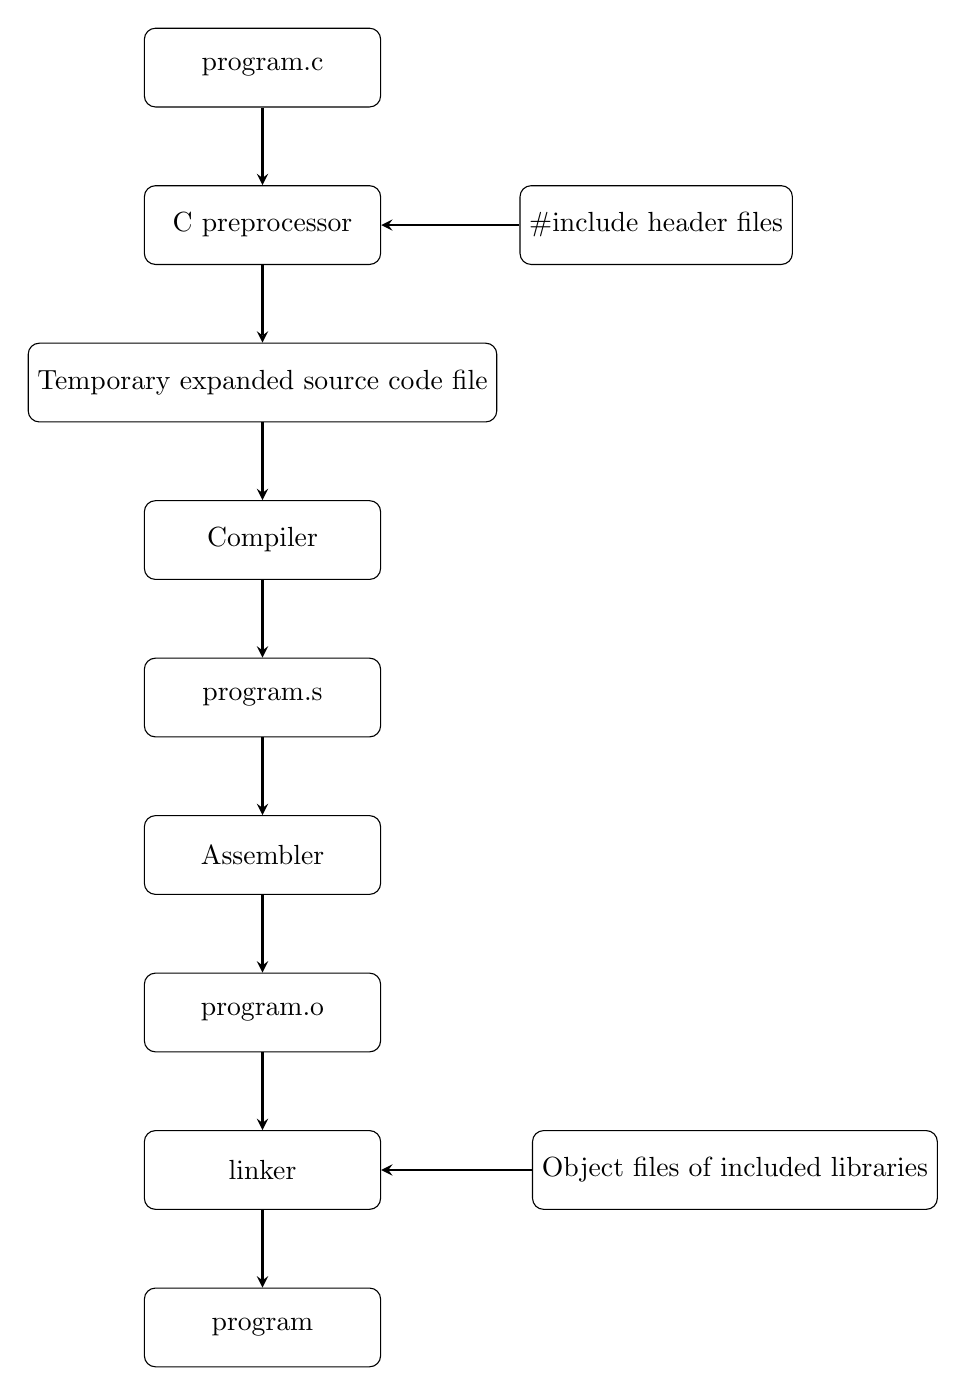
\begin{tikzpicture}[node distance=2cm]
	%defines
	\tikzstyle{programc} = [rectangle, rounded corners, minimum width=3cm, minimum height=1cm,text centered, draw=black]
	\tikzstyle{cPreProcessor} = [rectangle, rounded corners, minimum width=3cm, minimum height=1cm,text centered, draw=black]
	\tikzstyle{includeHeaderFiles} = [rectangle, rounded corners, minimum width=3cm, minimum height=1cm,text centered, draw=black]
	\tikzstyle{temporaryFile} = [rectangle, rounded corners, minimum width=3cm, minimum height=1cm,text centered, draw=black]
	\tikzstyle{compiler} = [rectangle, rounded corners, minimum width=3cm, minimum height=1cm,text centered, draw=black]
	\tikzstyle{programS} = [rectangle, rounded corners, minimum width=3cm, minimum height=1cm,text centered, draw=black]
	\tikzstyle{assembler} = [rectangle, rounded corners, minimum width=3cm, minimum height=1cm,text centered, draw=black]
	\tikzstyle{programO} = [rectangle, rounded corners, minimum width=3cm, minimum height=1cm,text centered, draw=black]
	\tikzstyle{linker} = [rectangle, rounded corners, minimum width=3cm, minimum height=1cm,text centered, draw=black]
	\tikzstyle{objectOfHeaders} = [rectangle, rounded corners, minimum width=3cm, minimum height=1cm,text centered, draw=black]
	\tikzstyle{program} = [rectangle, rounded corners, minimum width=3cm, minimum height=1cm,text centered, draw=black]
	\tikzstyle{arrow} = [thick,->,>=stealth]
	%chart
	\node (programc) [programc] {program.c};
	\node (cPreProcessor) [cPreProcessor, below of=programc] {C preprocessor};
	\node (includeHeaderFiles) [includeHeaderFiles, right of=cPreProcessor, node distance=5cm] {\#include header files};
	\node (temporaryFile) [temporaryFile, below of=cPreProcessor] {Temporary expanded source code file};
	\node (compiler) [compiler, below of=temporaryFile] {Compiler};
	\node (programS) [includeHeaderFiles, below of=compiler] {program.s};
	\node (assembler) [assembler, below of=programS] {Assembler};
	\node (programO) [programO, below of=assembler] {program.o};
	\node (linker) [linker, below of=programO] {linker};
	\node (objectOfHeaders) [objectOfHeaders, right of=linker, node distance=6cm] {Object files of included libraries};
	\node (program) [compiler, below of=linker] {program};
	\draw [arrow] (programc) -- (cPreProcessor);
	\draw [arrow] (includeHeaderFiles) -- (cPreProcessor);
	\draw [arrow] (cPreProcessor) -- (temporaryFile);
	\draw [arrow] (temporaryFile) -- (compiler);
	\draw [arrow] (compiler) -- (programS);
	\draw [arrow] (programS) -- (assembler);
	\draw [arrow] (assembler) -- (programO);
	\draw [arrow] (programO) -- (linker);
	\draw [arrow] (objectOfHeaders) -- (linker);
	\draw [arrow] (linker) -- (program);
\end{tikzpicture}